% !TEX root = main.tex

\section{Symbolic Execution Engines}
\label{se:executors}

In this section we describe some important principles for the design of symbolic executors as well as crucial tradeoffs that arise in their implementation. Moving from the concepts of concrete and symbolic runs, we also introduce the idea of ``concolic'' execution.

\subsection{Concrete, Symbolic, and Concolic Execution}
\label{ss:concrete-concolic-symbolic}

As shown in the warm-up example (Section~\ref{symbolic-execution-example}), a symbolic execution of a program can generate -- in theory -- all possible control flow paths that the program could take during its concrete executions on specific inputs. While modeling all possible runs allows for very interesting analyses, it is typically unfeasible in practice, especially on real-world software, for a variety of reasons.

First, as extensively discussed in Section~\ref{se:path-explosion}, the number of control flow paths to be generated and analyzed could be prohibitively large, due to branch instructions and loops. In the worst case, if the code contains an unbounded loop, symbolic execution could keep running forever, generating a potentially infinite number of paths (we refer to Section~\ref{se:loops} for an example).

Moreover, as observed in Section~\ref{se:intro}, symbolic engines are clients of SMT solvers, which are continuously invoked during the analysis. Although powerful SMT solvers are currently available, the time spent in constraint solving is still one of the main performance barriers for symbolic engines. It may also happen that the program yields constraints that the solver cannot handle well (e.g., non-linear constraints), in spite of the fact that symbolic executors often use more than one solver in order to support as many decidable logical fragments as possible.
%An SMT instance is a formula in first-order logic, where some function and predicate symbols have additional meaning. This meaning depends on the theory being used: for instance, with linear inequalities symbols with extra meaning include the integers, $+$, $-$, $x$, $\le$. Path constraints are typically expressed in a decidable logical fragment without quantifiers

\begin{figure}[t]
\centering

\includegraphics[width=0.35\columnwidth]{images/concrete-abstract.eps} 
\caption{Concrete and abstract execution machine models.}
\label{fig:concrete-symbolic}
\end{figure}

A standard approach to limit the resources (running time and space usage) required by the execution engine and to handle complex constraints is to mix concrete and symbolic execution: this is dubbed {\em concolic execution}, where the term concolic is a portmanteau of the words concrete and symbolic. The basic idea is to have the concrete execution drive the symbolic execution (see also Figure~\ref{fig:concrete-symbolic}). Besides the symbolic store and the path constraints, a concolic execution engine also maintains a concrete store $\sigma_c$. After choosing an arbitrary input to begin with, it executes the program both concretely and symbolically by simultaneously updating the two stores and the path constraints. In order to explore different paths, the path conditions given by one or more branches can be negated and the SMT solver invoked to find a satisfying assignment for the new constraints, i.e., to generate a new input.

%\mynote{[D] path conditions starting from the last one?}

%\begin{figure}[t]
%  \centering
%  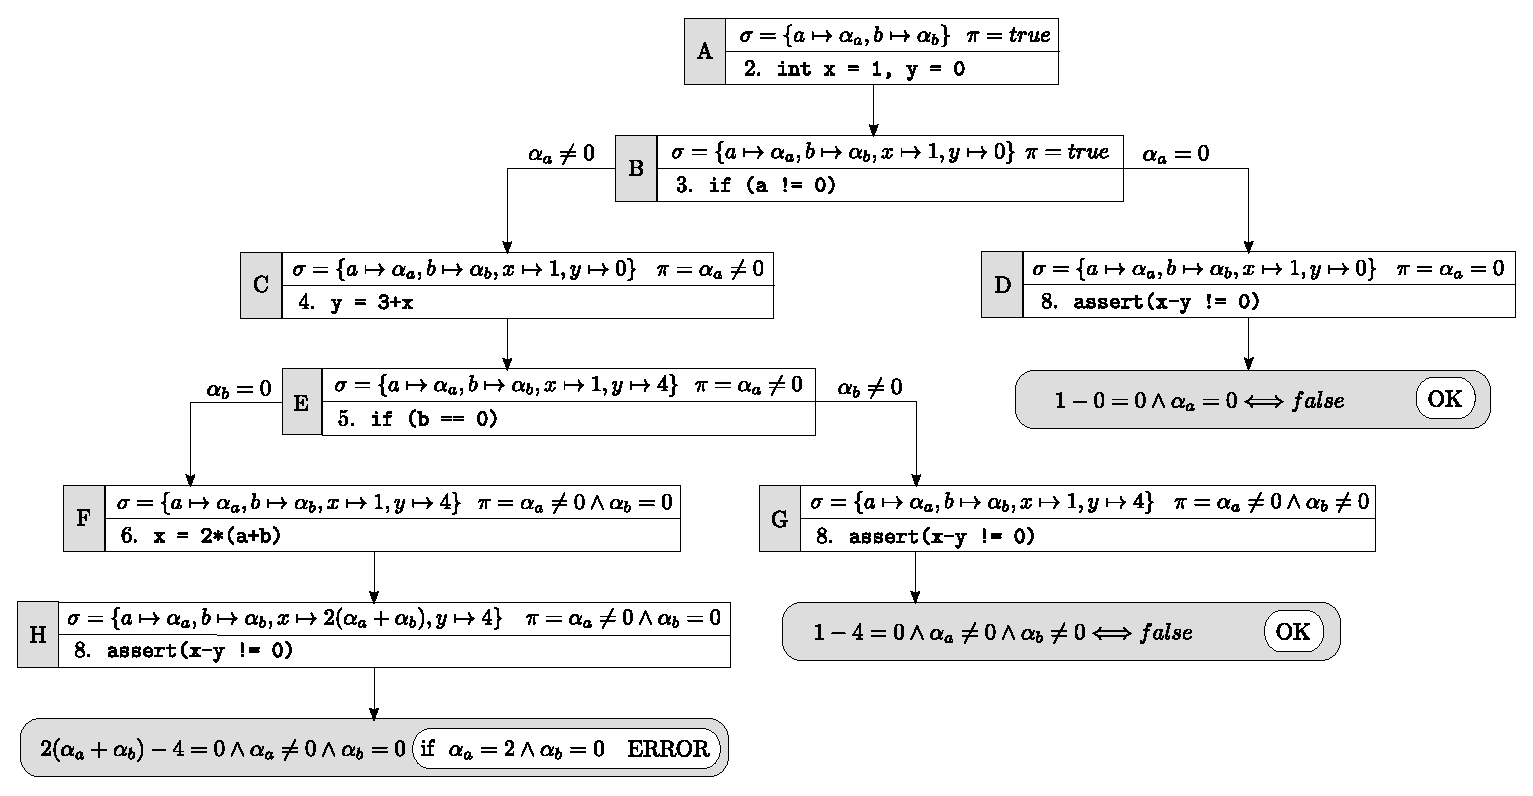
\includegraphics[width=1.0\columnwidth]{images/execution-tree.eps} 
%  \caption{TREE TO BE REPLACED. Concolic execution of function {\tt foobar} given in Figure~\ref{fig:example-1} starting with input $a = 1$ and $b = 1$. Besides the statement to be executed, the symbolic store $\sigma$, the path constraints $\pi$, execution states also show the concrete store $\sigma_c$. }
%%For the sake of presentation the conjunction of constraints is shown as a list of constraints. }
%  \label{fig:example-concolic-execution}
%\end{figure}

\boxedexample{
Consider the C function in Figure~\ref{fig:example-1} and suppose to choose $a = 1$ and $b = 1$ as input parameters. Under these conditions, the concrete execution takes path $A\leadsto B\leadsto C\leadsto E\leadsto G$ in the symbolic tree of Figure~\ref{fig:example-symbolic-execution}. Besides the symbolic stores shown in Figure~\ref{fig:example-symbolic-execution}, the concrete stores maintained in the traversed states are the following:
  \begin{enumerate}
  
  \item[]$-$~~$\sigma_c=\{a\mapsto 1,~b\mapsto 1\}$ in state $A$;
  \item[]$-$~~$\sigma_c=\{a\mapsto 1,~b\mapsto 1,~x\mapsto 1,~y\mapsto 0\}$ in states $B$ and $C$;
  \item[]$-$~~$\sigma_c=\{a\mapsto 1,~b\mapsto 1,~x\mapsto 1,~y\mapsto 4\}$ in states $E$ and $G$.
  
  \end{enumerate}  
%Stores and path constraints maintained by the concolic run are shown in Figure~\ref{fig:example-concolic-execution}. 
After checking that the \texttt{assert} conditions at line 8 succeed, we can generate a new control flow path by negating the last path constraint, i.e., $\alpha_b\neq 0$. The solver at this point would generate a new input that satisfies the constraints $\alpha_a\neq 0\,\wedge\, \alpha_b=0$ (for instance $a = 1$ and $b = 0$) and the execution would continue in a similar way along the path $A\leadsto B\leadsto C\leadsto E\leadsto F$. %
}

%\vspace{2mm}
%\noindent
%\fbox{%
%  \parbox{0.98\textwidth}{%
%  {\em Example.}  Consider the C function in Figure~\ref{fig:example-1} and suppose to choose $a = 1$ and $b = 1$ as input parameters. Under these conditions, the concrete execution takes path $A\leadsto B\leadsto C\leadsto E\leadsto G$ in the symbolic tree of Figure~\ref{fig:example-symbolic-execution}. Besides the symbolic stores shown in Figure~\ref{fig:example-symbolic-execution}, the concrete stores maintained in the traversed states are the following:
%  \begin{enumerate}
%  
%  \item[]$-$~~$\sigma_c=\{a\mapsto 1,~b\mapsto 1\}$ in state $A$;
%  \item[]$-$~~$\sigma_c=\{a\mapsto 1,~b\mapsto 1,~x\mapsto 1,~y\mapsto 0\}$ in states $B$ and $C$;
%  \item[]$-$~~$\sigma_c=\{a\mapsto 1,~b\mapsto 1,~x\mapsto 1,~y\mapsto 4\}$ in states $E$ and $G$.
%  
%  \end{enumerate}  
%%Stores and path constraints maintained by the concolic run are shown in Figure~\ref{fig:example-concolic-execution}. 
%After checking that the \texttt{assert} conditions at line 8 succeed, we can generate a new control flow path by negating the last path constraint, i.e., $\alpha_b\neq 0$. The solver at this point would generate a new input that satisfies the constraints $\alpha_a\neq 0\,\wedge\, \alpha_b=0$ (for instance $a = 1$ and $b = 0$) and the execution would continue in a similar way along the path $A\leadsto B\leadsto C\leadsto E\leadsto F$. }%
%}

\vspace{2mm}
\noindent As shown by the example, the symbolic information maintained during a concrete run can be exploited by the execution engine, for instance, to obtain new inputs and explore new control flow paths. We will further discuss this aspect in Section~\ref{ss:heuristics}. 

It is worth noticing that concolic execution trades soundness for performance: false negatives are indeed possible, because some program executions -- and therefore possible erroneous behaviors -- may be missed. In the literature, this is also regarded as an {\em under-approximate} form of program analysis.

% with fully symbolic phases, enabling program analysis across a full software stack without sacrificing scalability
Many papers exploit variants of concolic execution or different ways of mixing concrete and symbolic runs. For instance, in {\em execution-generated testing} (see, e.g., {\sc KLEE}~\cite{KLEE-OSDI08}, {\sc EXE}~\cite{EXE-CCS06}, and~\cite{CS-CACM13}, the symbolic engine always executes concretely the operations that involve only concrete values. This makes it possible to reason even over complex (e.g., non-linear) operations if they involve only concrete values. {\em Selective symbolic execution}~\cite{CKC-TOCS12} takes a different approach, by interleaving portions of code that are concretely run with fully symbolic phases. The interleaving must be done carefully in order to preserve the meaningfulness of the whole exploration. When an argument $x$ for a function call to concretize is symbolic, the engine should convert it to some concrete value in order to perform the call, which is equivalent to corseting the exploration to a single path in the callee. When the call returns and the symbolic phase resumes, the concrete value for $x$ becomes part of the path constraints for the remainder of the exploration. However, a large number of paths may be then excluded. {\sc \stwoe}~\cite{CKC-TOCS12} presents a systematic approach to consistently cross the symbolic/concrete boundary in both directions: it describes a strategy to deal with constraints introduced on symbolic values as a consequence of concretization, and introduces a number of consistency models -- where a state is {\em consistent} when there exists a feasible path to it from the initial state -- which suit different analyses. Constraints updated to account for concrete values are marked as {\em soft}, and whenever a branch in the symbolic domain is disabled because of a soft constraint, execution goes back and picks a value for the concrete call that would enable that branch. Throughout the paper we will see other uses of concretization (see, e.g., Section~\ref{memory-model} and Section~\ref{se:constraint-solving})  and of concolic execution (see Section~\ref{se:path-explosion}).


%===================================================================================
\subsection{Design Principles of Symbolic Executors}
\label{ss:principles}

A number %\mynote{[D] why MAYHEM?}  
of performance-related design principles that a symbolic execution engine should follow are  summarized in %{\sc Mayhem}
\cite{MAYHEM-SP12}. Most notably:
\begin{enumerate}
  \item {\em Progress}: the executor should be able make forward progress for an arbitrarily long time without exceeding the given resources. Memory consumption is especially critical, due to the gargantuan number of control flow paths.
  \item {\em Work repetition}: no execution work should be repeated, avoiding to restart a program several times from its very beginning in order to analyze different paths that might have a  common prefix.
  \item {\em Analysis reuse}: analysis results from previous runs should be reused as much as possible. In particular, costly invocations to the SMT solver on  previously solved path constraints should be avoided.
\end{enumerate}

\noindent Due to the large size of the execution state space to be analyzed, different symbolic engines have explored different tradeoffs between, e.g., running time and memory consumption, or performance and soundness/completeness of the analysis.

Symbolic executors that try to execute multiple paths in parallel in a single run -- also called {\em online executors} -- clone the execution state at each input-dependent branch. Examples are given in {\sc KLEE}~\cite{KLEE-OSDI08}, {\sc AEG}~\cite{AEG-NDSS11}, {\sc \stwoe}~\cite{CKC-TOCS12}. These engines never re-execute previous instructions, thus avoiding work repetition. However, since many active states need to be kept in memory, they put a huge burden on memory consumption, possibly hindering progress. Moreover, executing multiple paths in parallel requires to ensure isolation between execution states, e.g., keeping different states of the OS by emulating the effects of system calls.

Reasoning about a single path at a time, as in concolic execution, is the approach taken by so-called {\em offline executors}, such as {\sc SAGE}~\cite{SAGE-NDSS08}. Running each path independently of the others results in low memory consumption with respect to online executors and in the capability of reusing immediately analysis results from previous runs. On the other side, the work can be largely repeated, since each run typically restarts the execution of the program from the very beginning. In a typical implementation of offline executors, runs are concrete and require an input seed: the program is first executed concretely, a trace of instructions is recorded, and the recorded trace is then executed symbolically.

{\em Hybrid executors} such as {\sc Mayhem}~\cite{MAYHEM-SP12} attempt at  balancing between speed and memory requirements: they start in online mode and generate checkpoints, rather than forking new executors, when memory usage or the number of concurrently active states reaches a threshold. Checkpoints maintain the symbolic execution state and replay information. When a checkpoint is picked for restoration, the concrete state is restored and the online exploration resumes.
%: mixed approach. Start with an online approach, if needed switch to offline mode by doing checkpoints. A checkpoint contains the symbolic execution state and replay information. Concrete execution state is discarded since it can be quickly recovered at runtime by using one input generated by the solver before checkpointing.

%===================================================================================
\subsection{Caching} 
\label{ss:caching}

Caching is a powerful technique to achieve time-space tradeoffs and is embodied in symbolic executors in different ways. Most prominently:

\begin{itemize}

\item {\em Function caching.} A function $f$, and more in general any part of a program, may be called multiple times during an execution, either at the same calling context or at different ones. The traditional symbolic execution approach requires to symbolically execute $f$ at each call. \cite{G-POPL07} proposes a compositional approach that dynamically generates {\em function summaries}, allowing the symbolic executor to effectively reuse prior discovered analysis results. A similar idea has been also proposed in~\cite{BCE-TACAS08}. The main intuition is that, if two program states differ only for some program values that are not read later, the executions generated by the two program states will produce the same side effects. Side effects of a portion of code can be therefore cached and possibly reused later. 

%Since the two techniques are almost equivalent, our discussion will follow~\cite{G-POPL07}. 
%\paragraph{Definition of function summaries} A function summary $\phi_f$ for a function $f$ is defined as a propositional logic formula. It can be computed by successive iterations and defined as a disjunction of formulas $\phi_w$ of the form $\phi_w = {pre}_w \wedge post_w$, where $w$ is a possible execution path of function $f$, $pre_w$ is a conjunction of constraints over the inputs of $f$, and $post_w$ is a conjunction of constraints over the outputs of $f$. Formally, $\phi_f = \bigvee \phi_w$.  
%
%\paragraph{Using function summaries} Whenever a function $f$ is called, the symbolic execution engine checks whether a summary $\phi_w$ of $f$ with $pre_w$ compliant with the current path constraints is available. If so, the post conditions $post_w$ are added to the current symbolic state. Otherwise, if no matching summary is found, a new function summary is computed.
%
%\paragraph{Computing function summaries} Function summaries can be computed dynamically: whenever there is an invocation of a function $f$, $pre_w$ is obtained from the current set of constraints over the input of $f$, while $post_w$ is given by tracking constraints over the \mynote{[D] no symbolic?}concolic\footnote{{\em [D] If this technique applies to concolic executors only we should say it upfront!}} execution of function $f$ over some concrete inputs that are compliant with $pre_w$. Notice that $pre_w$ defines an equivalence class of concrete executions that result in executions characterized by $post_w$. 
%
%\paragraph{Issues} If the symbolic execution engine cannot reason on one or more statements contained in a function $f$, then the generated summary cannot be \mynote{[D] blindly}blindly reused. For instance, consider a function that contains a call to an external function (e.g., a system call) or to a {\em complex} one (e.g., a hash function). In this scenario, even if a matching function summary is found, the related post conditions $post_w$ may not be valid since they have been generated over a concrete execution and thus cannot be generalized. % robust hash function

\item {\em Loop summarization.} In order to avoid redundant executions of the same loop under the same program state, loop summaries can be computed and cached for later reuse, similarly to function summaries. We refer to Section~\ref{se:loops} for details on a loop summarization strategy proposed in~\cite{GL-ISSTA11}.

\item {\em Constraint reuse.} In order to speed up constraint solving, different works support the reuse of constraint  solutions based on syntactic or semantic equivalence of the constraints. Examples are given in {\sc EXE}~\cite{EXE-CCS06}, {\sc KLEE}~\cite{KLEE-OSDI08}, and~\cite{MEMO-ISSTA12,GREEN-FSE12}. We will further discuss this optimization in Section~\ref{se:constraint-solving}.

\end{itemize}


\subsection{Tools}

Table~\ref{tab:symbolic-engines} lists a number of symbolic execution engines that have worked as incubators for several of the techniques surveyed in this article. The novel contributions introduced by tools that represented milestones in the area are described in the appropriate sections throughout the paper.

\begin{figure}[t]
  \centering
  \begin{adjustbox}{width=1\columnwidth}
  %\begin{small}
  \begin{tabular}{| l || c || l |}
    \hline      
    {\bf Symbolic engine} & {\bf References} & {\bf Project URL} (last retrieved: August 2016)  \\ \hline\hline
    
    % CNC is not a symbolic engine but it uses constrained solver
    %{\sc Check 'n' Crash} & \cite{CS-ICSE05} & \url{http://ranger.uta.edu/~csallner/cnc/}\\
    
    {\sc CUTE} & \cite{CUTE-FSE13} & -- \\
    {\sc DART} & \cite{DART-PLDI05} & -- \\
    {\sc jCUTE} & \cite{SA-CAV06} & \url{https://github.com/osl/jcute} \\ % : Java Concolic Unit Testing Engine
    {\sc KLEE} & \cite{EXE-CCS06,KLEE-OSDI08} & \url{https://klee.github.io/} \\ % : a LLVM Execution Engine
    {\sc SAGE} & \cite{SAGE-NDSS08,EGL-ISSTA09} & -- \\
    {\sc BitBlaze} & \cite{BITBLAZE-ICISS08} & \url{http://bitblaze.cs.berkeley.edu/} \\ % , BHK-TR07
    {\sc CREST} & \cite{CREST-ASE08} & \url{https://github.com/jburnim/crest} \\ % : a concolic test generation tool for C
    {\sc PEX} & \cite{PEX-TAP08} & \url{http://research.microsoft.com/en-us/projects/pex/} \\
    {\sc Rubyx} & \cite{CF-CCS10} & -- \\
    {\sc Java PathFinder} & \cite{PATHFINDER-ASE10} & \url{http://babelfish.arc.nasa.gov/trac/jpf}\\
    {\sc Otter} & \cite{RSM-ICSE10} & \url{https://bitbucket.org/khooyp/otter/} \\
    {\sc BAP} & \cite{BAP-CAV11} & \url{https://github.com/BinaryAnalysisPlatform/bap} \\
    {\sc Cloud9} & \cite{CLOUD9-EUROSYS11} & \url{http://cloud9.epfl.ch/} \\
    {\sc Mayhem} & \cite{MAYHEM-SP12} & -- \\
    {\sc SymDroid} & \cite{JMF-TECH12} & -- \\
    {\sc \stwoe} & \cite{CKC-TOCS12} & \url{http://s2e.epfl.ch/} \\
    {\sc FuzzBALL} & \cite{MMP-ASPLOS12,FUZZBALL-ESORICS13} & \url{http://bitblaze.cs.berkeley.edu/fuzzball.html} \\
    {\sc Jalangi} & \cite{SKB-FSE13} & \url{https://github.com/Samsung/jalangi2} \\
    {\sc Pathgrind} & \cite{S-ICSE04} & \url{https://github.com/codelion/pathgrind} \\
    {\sc Kite} & \cite{V-THESIS14} & \url{http://www.cs.ubc.ca/labs/isd/Projects/Kite} \\
    {\sc SymJS} & \cite{LAG-FSE14} & -- \\
    {\sc CIVL} & \cite{CIVL-SC15} & \url{http://vsl.cis.udel.edu/civl/}\\ % : The Concurrency Intermediate Verification Language 
	{\sc KeY} & \cite{HBR-RV14} & \url{http://www.key-project.org/} \\
    {\sc Angr} & \cite{FIRMALICE-NDSS15,ANGR-SSP16} & \url{http://angr.io/} \\
    {\sc Triton} & \cite{TRITON-SSTIC15} & \url{http://triton.quarkslab.com/} \\
    {\sc JDart} & \cite{JDART-TACAS16} & \url{https://github.com/psycopaths/jdart} \\

    {\sc CATG} & -- & \url{https://github.com/ksen007/janala2} \\
    {\sc PySymEmu} & -- & \url{https://github.com/feliam/pysymemu/} \\
    {\sc Miasm} & -- & \url{https://github.com/cea-sec/miasm} \\
    
    \hline  
  \end{tabular}
  %\end{small}
  \end{adjustbox}
  \caption{A selection of symbolic execution engines, along with their reference article and software project web site (if any).}
  \label{tab:symbolic-engines}
\end{figure}

